% Robot-Whisper 汇报 PPT
% 编译:pdflatex -interaction=nonstopmode robot-whisper.tex  (跑两遍出页码)
% 中文:CJKutf8 + Arphic gbsn(与 latex-next-live 项目同一工具链)
\documentclass[aspectratio=169,10pt]{beamer}
\usepackage{CJKutf8}
\usepackage{graphicx}
\usepackage{booktabs}
\usepackage{array}
\usepackage{amsmath}
\usepackage{tikz}
\usetikzlibrary{arrows.meta,positioning}

\AtBeginDocument{\begin{CJK*}{UTF8}{gbsn}}
\AtEndDocument{\clearpage\end{CJK*}}

%==================== 主题 ====================
\usetheme{default}
\usecolortheme{default}
\setbeamertemplate{navigation symbols}{}

\definecolor{teal}{RGB}{12,110,97}
\definecolor{gold}{RGB}{140,94,14}
\definecolor{brick}{RGB}{172,55,43}
\definecolor{ink}{RGB}{29,26,20}
\definecolor{paper}{RGB}{247,244,236}
\definecolor{gray2}{RGB}{110,103,87}

\setbeamercolor{normal text}{fg=ink,bg=paper}
\setbeamercolor{frametitle}{fg=teal,bg=paper}
\setbeamercolor{title}{fg=teal}
\setbeamercolor{structure}{fg=teal}
\setbeamercolor{itemize item}{fg=gold}
\setbeamercolor{itemize subitem}{fg=gray2}
\setbeamerfont{frametitle}{size=\large,series=\bfseries}
\setbeamertemplate{itemize item}{\textbullet}
\setbeamertemplate{itemize subitem}{--}

% 页脚:左=题名 右=页码
\setbeamertemplate{footline}{%
  \hbox{\begin{beamercolorbox}[wd=\paperwidth,ht=2.4ex,dp=1.4ex,leftskip=.9em,rightskip=.9em]{}%
    {\scriptsize\color{gray2}Robot-Whisper\hfill\insertframenumber}%
  \end{beamercolorbox}}}

% 小工具
\newcommand{\hi}[1]{{\color{teal}\bfseries #1}}
\newcommand{\wi}[1]{{\color{gold}\bfseries #1}}
\newcommand{\bad}[1]{{\color{brick}\bfseries #1}}
\newcommand{\dimm}[1]{{\footnotesize\color{gray2}#1}}
\newcommand{\lead}[1]{{\large\color{teal}#1}\par\medskip}
\newcommand{\warn}[1]{{\footnotesize\color{brick}$\triangleright$~#1}}

\title{Neurons see the state the tokens don't}
\subtitle{具身智能的内生异常警报}
\author{Robot-Whisper}
\date{}

\begin{document}

%==================================================== P1 封面
{\setbeamercolor{background canvas}{bg=paper}
\begin{frame}[plain]
  \vspace{1.1cm}
  \begin{center}
    {\LARGE\color{teal}\bfseries 神经元看到了 token 看不到的状态}\\[4pt]
    {\LARGE\color{gold}\bfseries 具身场景下的异常警报}\\[16pt]
    {\color{gray2}\rule{7cm}{0.4pt}}\\[12pt]
    {\small VLA \quad$\cdot$\quad LIBERO-10 \quad$\cdot$\quad 864 rollouts \quad$\cdot$\quad 四个事先冻结的常数}\\[18pt]
    \colorbox{white}{\parbox{0.72\textwidth}{\centering\vspace{3pt}\small
      手还在动,事情已经不对了 —— 最早知道的,不是画面,也不是动作,\\
      是模型深处的神经元。\vspace{3pt}}}\\[18pt]
    {\footnotesize\color{gray2}向内探寻,向外进化\qquad Seek within. Evolve beyond.}
  \end{center}
\end{frame}}

%==================================================== P2 起点
\begin{frame}{起点:一件旧事}
  \lead{内部状态知道的,比 token 说出来的多。}
  \begin{itemize}
    \item 推理大模型上的探针 \hi{NAD}:在多条候选答案之间,\textbf{不读一个字},
          只凭神经元活动就能挑出更可能对的那条
    \item 把握与犹豫没有写进 token,但内部状态里有
  \end{itemize}
  \vfill
  \begin{center}
    \colorbox{white}{\parbox{0.86\textwidth}{\centering\vspace{2pt}
      \large 同一个思想换到具身场景 ——\\[3pt]
      \wi{VLA 大模型的内部,会不会也有类似的信号?}\vspace{4pt}}}
  \end{center}
  \vfill
  \dimm{Chen et al., 2025 · Neuron Agreement Decoding · ICML 2026 Spotlight}
\end{frame}

%==================================================== P3 现象
\begin{frame}{现象:两条只差一条噪声的轨迹}
  \begin{columns}[T]
    \column{0.5\textwidth}\centering
      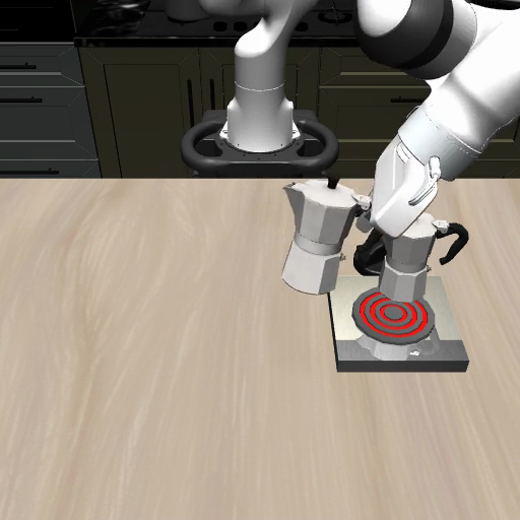
\includegraphics[width=\linewidth]{figs/succ.png}\\[3pt]
      {\color{teal}\bfseries $\checkmark$ 两只壶先后上炉}\\ \dimm{38 步 $\cdot$ 18.6 s}
    \column{0.5\textwidth}\centering
      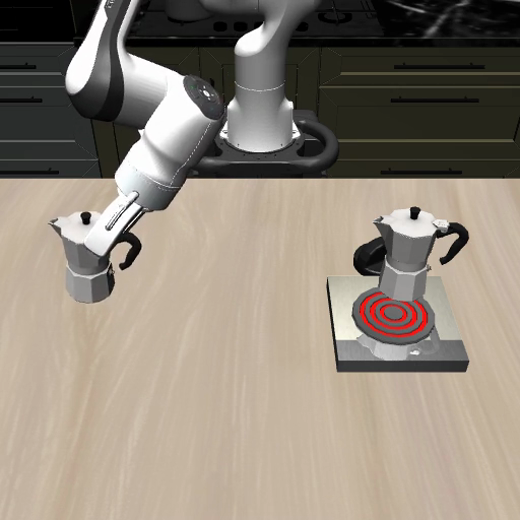
\includegraphics[width=\linewidth]{figs/fail.png}\\[3pt]
      {\color{brick}\bfseries $\times$ 悬在第二只壶上方}\\ \dimm{52 步 $\cdot$ 26.0 s $\cdot$ 超时}
  \end{columns}
  \vfill
  \begin{center}
  同一个模拟器状态,唯一的区别是扩散头的\hi{一条采样噪声}。\\[4pt]
  \wi{分开它们的那件事,从未出现在任何 token 里。}
  \end{center}
\end{frame}

%==================================================== P4 物理 trap
\begin{frame}{物理世界的 trap 长什么样}
  \begin{columns}[T]
    \column{0.62\textwidth}
      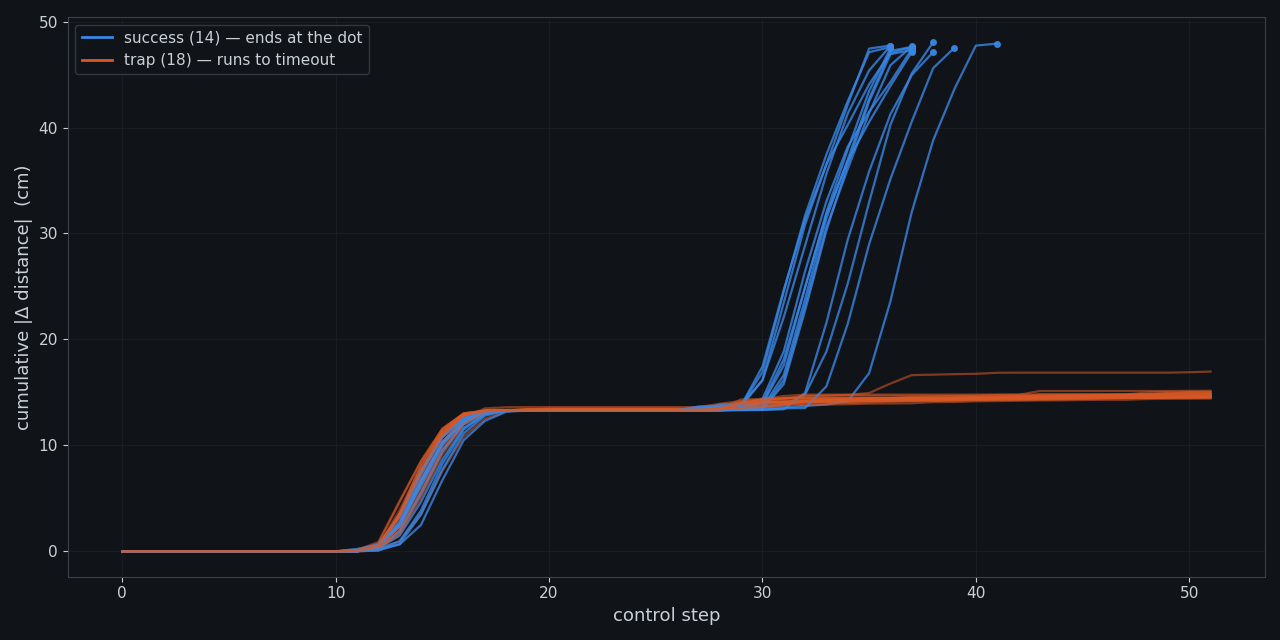
\includegraphics[width=\linewidth]{figs/fig_trap.png}
    \column{0.36\textwidth}
      \small
      固定同一初始状态,只变采样噪声,跑 32 条:\\[2pt]
      \hi{14 成功} \quad / \quad \bad{18 超时}\\[8pt]
      纵轴是\textbf{累计变化量},不是到目标距离 ——\\
      \dimm{有的 trap 就停在目标旁边}\\[8pt]
      前半段同路:放好第一只壶(+13 cm),一起歇脚\\[6pt]
      \wi{分岔在第 30 步}:蓝色重新起跳;\\
      橙色\textbf{再也没涨过一厘米}
  \end{columns}
  \vfill
  \begin{center}\small 世界还在被改变,曲线就还在涨。\end{center}
\end{frame}

%==================================================== P5 token 侧的局限
\begin{frame}{为什么 token / 动作侧难办}
  \vspace{2mm}
  \begin{columns}[T]
    \column{0.31\textwidth}
      {\color{gold}\bfseries 01\quad 动作流照常输出}\\[4pt]
      \small 每个卡住的步,模型照样吐出幅值正常的 10 帧动作
    \column{0.31\textwidth}
      {\color{gold}\bfseries 02\quad 判决在终点}\\[4pt]
      \small 成功要等布尔判定翻真;而“长”两解 —— 慢成功和快失败读起来一样
    \column{0.31\textwidth}
      {\color{gold}\bfseries $\rightarrow$\quad 得去别处看}\\[4pt]
      \small 悬停也好、打转也好,动作序列上读不出\textbf{分类}
  \end{columns}
  \vfill
  \begin{center}
  \colorbox{white}{\parbox{0.9\textwidth}{\small\vspace{2pt}
    \warn{口径提醒:动作侧\textbf{能}分成败(动作幅值 t=30 AUC 0.832),
    但它读的是\textbf{任务阶段}而非卡住 —— 详见防御页 D1--D2。}\vspace{2pt}}}
  \end{center}
\end{frame}

%==================================================== P6 神经元
\begin{frame}{神经元:pattern 与它的动力学}
  \begin{columns}[T]
    \column{0.55\textwidth}
      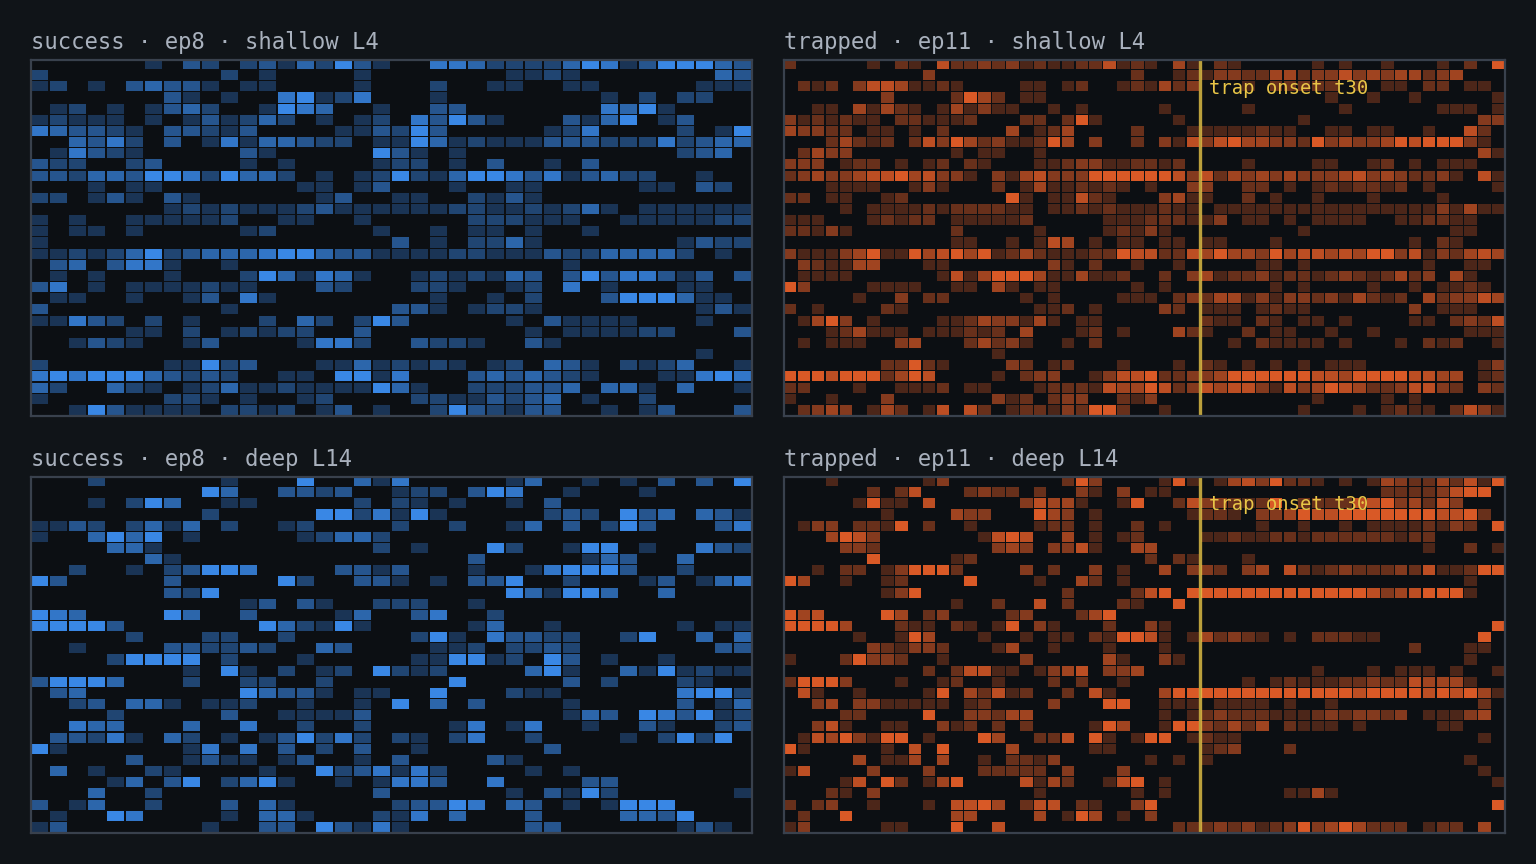
\includegraphics[width=\linewidth]{figs/fig_heat.png}
    \column{0.43\textwidth}
      \small
      每个控制步,模型点亮一小撮神经元\\
      \dimm{4 个深层 $\times$ 11 个动作 token}\\[6pt]
      先试了读\textbf{身份}(谁被点亮):\bad{没用}\\
      \dimm{身份是场景指纹,换初始状态整套重排}\\[8pt]
      有意义的是它的\hi{动力学}:\\
      顺利时随世界更迭,受困时更迭\textbf{变慢}\\[10pt]
      \colorbox{white}{\parbox{0.95\linewidth}{\centering\vspace{2pt}
        \wi{信号不在内容里,在流动里}\vspace{2pt}}}
  \end{columns}
  \vfill
  \dimm{金线 t30 之后,右下角拉出水平条纹。实测:持久专家 0.27/4,是\emph{换手速度降三分之一},不是完全冻结。}
\end{frame}

%==================================================== P7 三步
\begin{frame}{把凝固做成警报:三步}
  \small
  \begin{columns}[T]
    \column{0.3\textwidth}
      {\color{gold}\bfseries $d_s$\ \ 这一步挪了多远}\\[4pt]
      相邻两步点亮集合的重叠距离 $1-|\cap|/|\cup|$,平均成一个数
    \column{0.3\textwidth}
      {\color{gold}\bfseries $r(t)$\ \ 和自己比}\\[4pt]
      除以\textbf{自己开头 8 步}:只回答“我比刚出发时慢了多少”
    \column{0.34\textwidth}
      {\color{gold}\bfseries $\theta\cdot K$\ \ 何时拉响}\\[4pt]
      连续 $K{=}3$ 步 $r(t)<0.95$ $\rightarrow$ 报警。四个常数在救援实验\textbf{之前}冻结
  \end{columns}
  \vfill
  \begin{center}
    $\displaystyle r(t)=\frac{W^{-1}\sum_{s=t-W+1}^{t} d_s}{W_0^{-1}\sum_{s=1}^{W_0} d_s},
     \qquad W=4,\quad W_0=8$
  \end{center}
  \vfill
  \begin{center}
  \colorbox{white}{\parbox{0.88\textwidth}{\centering\small\vspace{2pt}
    为什么要除以自己:变化水位的方差 \wi{66.8\%} 由场景决定($\eta^2{=}0.668$),
    自归一扣掉的正是这 67\%。\vspace{2pt}}}
  \end{center}
\end{frame}

%==================================================== P8 相空间
\begin{frame}{相空间:三种命运}
  \begin{columns}[T]
    \column{0.58\textwidth}
      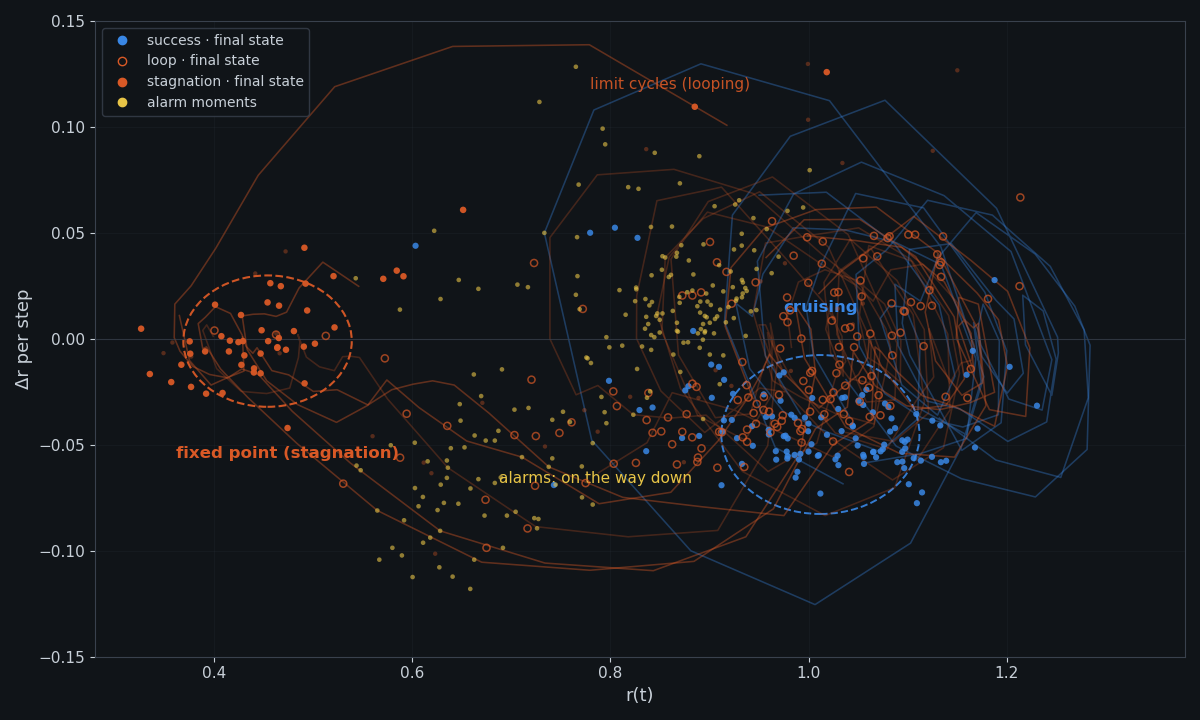
\includegraphics[width=\linewidth]{figs/fig_phase.png}
    \column{0.4\textwidth}\small
      \begin{tabular}{@{}ll@{}}
        \toprule
        \textbf{区域} & \textbf{对应} \\ \midrule
        巡航 & 正常干活,$r\approx 1.0$ \\
        不动点 & 停滞类,$r\approx 0.45$ \\
        极限环 & 打转类,一直在动 \\ \bottomrule
      \end{tabular}\\[10pt]
      后期阻尼比实测:\\
      停滞 $\zeta=0.83$ \ vs \ 打转 $\zeta=0.31$\\
      同场景内 AUC \hi{0.651}\\[8pt]
      \bad{极限环那一族}终态混进巡航区 ——\\ 是漏报的主要来源
  \end{columns}
\end{frame}

%==================================================== P9 结果
\begin{frame}{结果:抓住八成失败}
  \vspace{3mm}
  \begin{center}
  \begin{tabular}{@{}c@{\hskip 1.4cm}c@{\hskip 1.4cm}c@{}}
    {\Huge\color{teal}\bfseries 81.2\%} & {\Huge\color{gold}\bfseries +19.7} & {\Huge\color{teal}\bfseries 80\%}\\[4pt]
    \dimm{在线判对 $\cdot$ 864 条} & \dimm{高出多数类基线(61.5\%)} & \dimm{失败召回 $\cdot$ 误报 17\%}\\
  \end{tabular}
  \end{center}
  \vfill
  \begin{columns}[T]
    \column{0.48\textwidth}\centering
      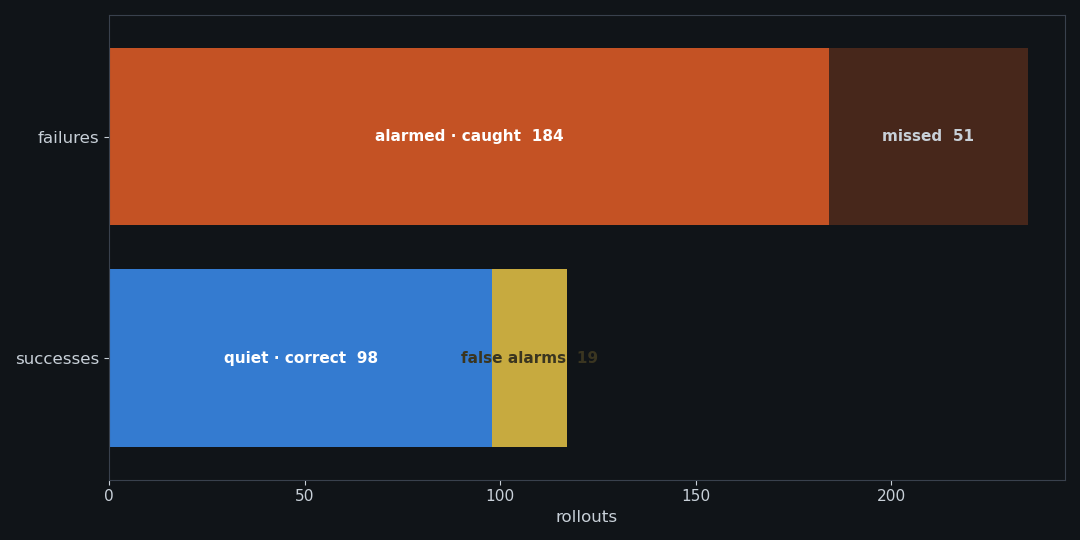
\includegraphics[width=\linewidth]{figs/fig_outcome.png}\\
      \dimm{判决矩阵:失败 235 抓住 184,成功 117 误伤 19}
    \column{0.48\textwidth}\centering
      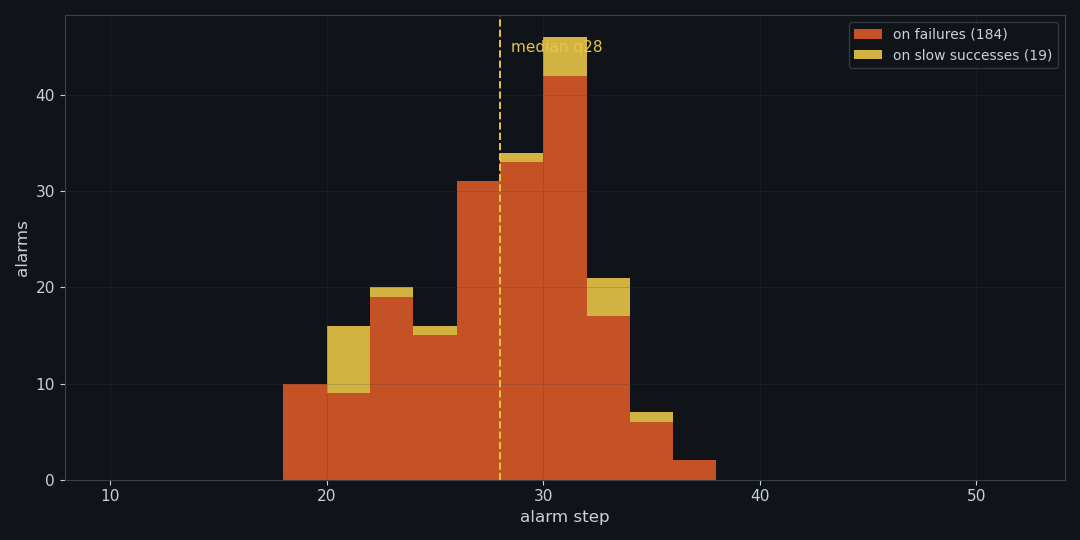
\includegraphics[width=\linewidth]{figs/fig_alarmtime.png}\\
      \dimm{报警落点 q18--q36,中位 q28 —— 距超时还有一半路程}
  \end{columns}
  \vfill
  \begin{center}\small 跨\textbf{不同任务、不同初始状态};不看画面、不看动作、不看任务标签。\end{center}
\end{frame}

%==================================================== P10 误报
\begin{frame}{误报是什么}
  \begin{columns}[T]
    \column{0.52\textwidth}
      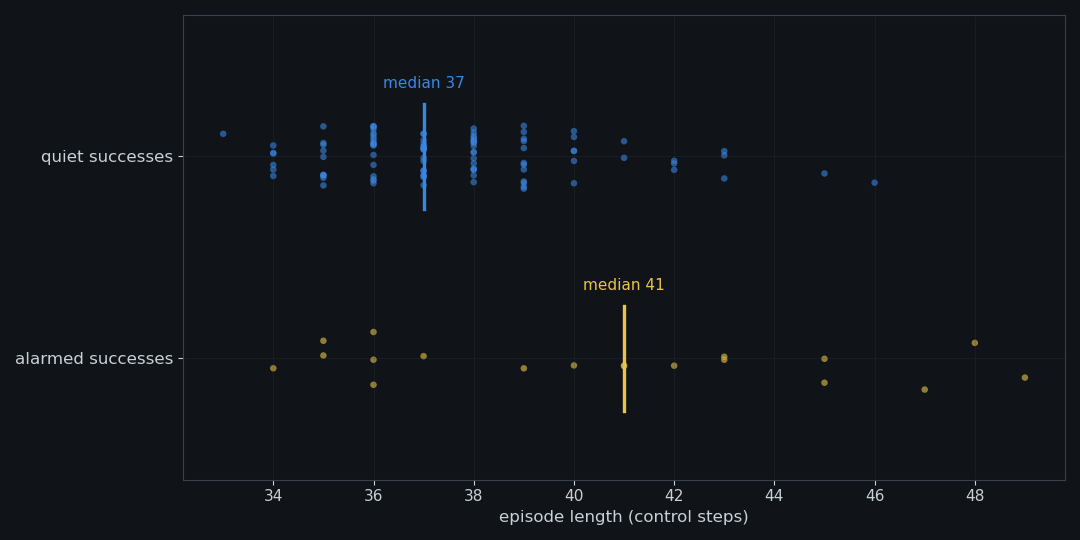
\includegraphics[width=\linewidth]{figs/fig_slow.png}
    \column{0.44\textwidth}\small
      被误报的成功中位 \wi{41 步},\\
      安静的成功中位 \hi{37 步}\\[6pt]
      它们确实\textbf{更慢} —— 减速、擦着不动点的引力边缘,又自己爬回巡航区\\[10pt]
      \colorbox{white}{\parbox{0.95\linewidth}{\centering\vspace{2pt}
        警报读作 \wi{“正在下坠”}\\ 而不是“必然坠毁”\vspace{2pt}}}\\[8pt]
      \dimm{这也是急救实验采用的读法}
  \end{columns}
\end{frame}

%==================================================== P11 机制:环锁死
\begin{frame}{机制:不是模型坏了,是环锁死了}
  \vspace{1mm}
  \begin{columns}[c]
    \column{0.46\textwidth}
      \centering
      \begin{tikzpicture}[>=Latex,font=\small,
          bx/.style={draw,rounded corners,fill=white,minimum width=22mm,minimum height=8mm}]
        \node[bx] (m) at (0,2.1) {模型};
        \node[bx] (w) at (2.1,0) {世界};
        \node[bx] (o) at (-2.1,0) {观测};
        \draw[->,teal,very thick] (o) -- (m);
        \draw[->,teal,very thick] (m) -- node[right,font=\scriptsize,xshift=1mm]{动作} (w);
        \draw[->,brick,very thick] (w) -- node[below,font=\scriptsize,align=center]{任务状态\\不再改变} (o);
        \node[font=\scriptsize,color=gray2] at (0,0.85) {锁死};
        \draw[->,brick,thick,dashed] (0.75,0.85) arc (0:300:0.75);
      \end{tikzpicture}
    \column{0.5\textwidth}\small
      \textbf{没有任何一个零件坏掉}\\[3pt]
      模型正确响应了输入,物理也没错 ——\\
      是\hi{复合映射有一个不是目标的不动点}\\[9pt]
      \textbf{为什么模型抓不到}(policy\_input 实证):\\[3pt]
      \colorbox{white}{\parbox{0.95\linewidth}{\scriptsize\vspace{2pt}
        \texttt{image (224,224,3)}\\
        \texttt{wrist\_image (224,224,3)}\\
        \texttt{state (8,)}\\[2pt]
        \bad{没有一个维度是时间。}\vspace{2pt}}}
  \end{columns}
  \vfill
  \dimm{三层障碍:① 输入无历史(π0/OpenVLA 类)② 演示数据里没有失败(所有模仿学习)③ 卡住时历史窗口内全是同一帧}
\end{frame}

%==================================================== P12 语义层
\begin{frame}{失效在语义层,不在动力学层}
  \small
  \begin{columns}[T]
    \column{0.46\textwidth}
      \begin{tabular}{@{}p{1.5cm}p{4.2cm}@{}}
        \toprule
        \textbf{层} & \textbf{内容} \\ \midrule
        动力学 & $s'=f(s,a)$ 动作有没有产生预期的物理效果 \emph{(能学)} \\[3pt]
        \bad{语义} & $\Delta\phi(s)$ 这个效果有没有让任务前进 \emph{(需目标监督)} \\ \bottomrule
      \end{tabular}\\[10pt]
      \colorbox{white}{\parbox{0.95\linewidth}{\vspace{2pt}
        手臂照常移动 \wi{3.3 cm/chunk},效率还高 4.8\%。\\
        净/路程 0.52,远高于随机游走 0.29 ——\\
        \textbf{大跨度、有方向地做无用功。}\vspace{2pt}}}
    \column{0.5\textwidth}
      \begin{tabular}{@{}lr@{}}
        \toprule
        \textbf{失败 rollout,卡住前$\rightarrow$后} & \textbf{变化} \\ \midrule
        指令幅值        & $-5.4\%$ \\
        末端路程        & \hi{$+10\%$} \\
        末端净位移      & \hi{$+7\%$} \\
        回转半径        & \hi{$+17\%$} \\
        执行效率(位移/指令) & \hi{$+4.8\%$} \\ \midrule
        \bad{任务进展}  & \bad{$-100\%$} \\ \bottomrule
      \end{tabular}
  \end{columns}
  \vfill
  \dimm{推论:所有只学 $p(s'|s,a)$ 的模型(世界模型/卡尔曼/逆动力学)在这类 trap 里预测得非常准,新息 $\approx 0$。本项目卡尔曼实测 0.69--0.71,输给基线 0.799。}
\end{frame}

%==================================================== P13 急救
\begin{frame}{急救!!\quad 报警那一步,做一下干预}
  \begin{columns}[T]
    \column{0.5\textwidth}
      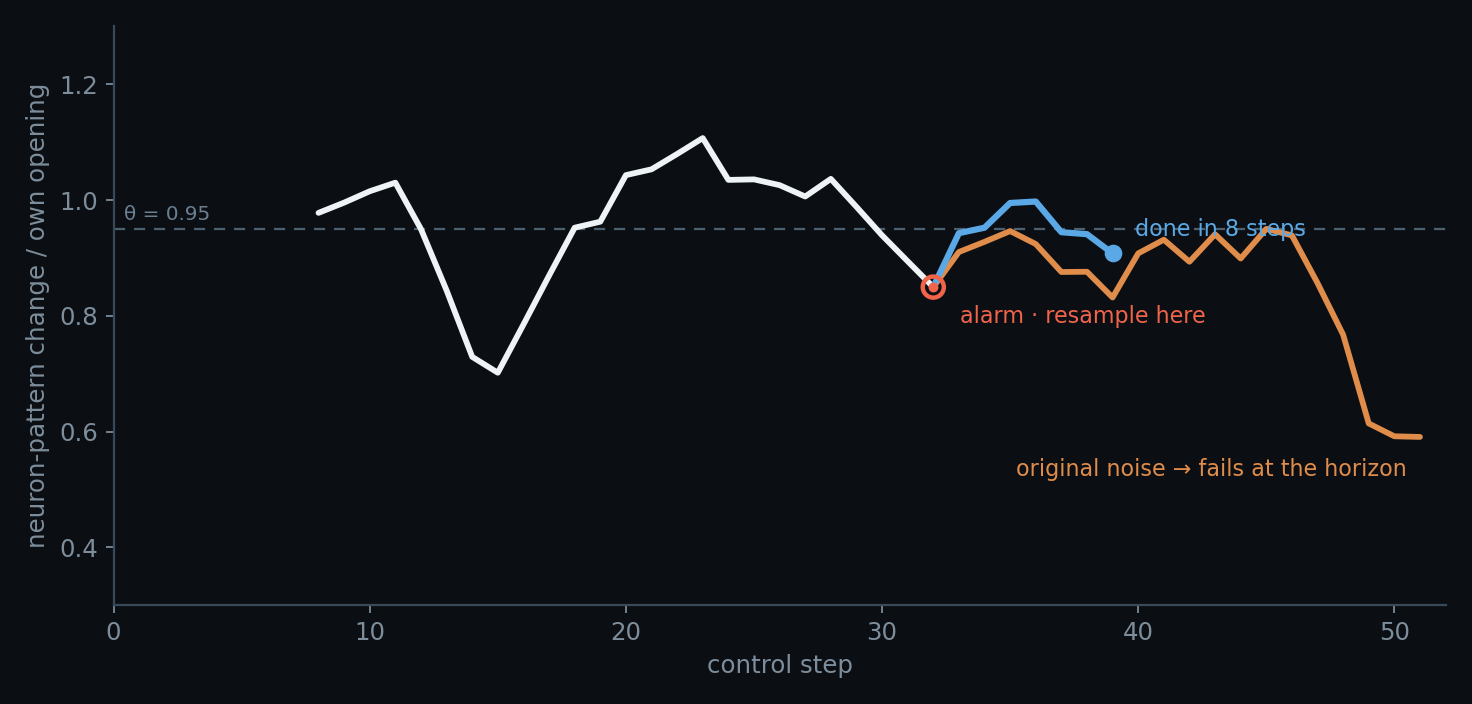
\includegraphics[width=\linewidth]{figs/fig_rescue.png}
    \column{0.46\textwidth}\small
      q32 报警 $\rightarrow$ \textbf{冻结状态} $\rightarrow$ 只加一点干扰
      (大幅度改换采样噪声)$\rightarrow$ 继续。其余一切不动。\\[8pt]
      \begin{tabular}{@{}lr@{}}
        \toprule
        救回 & \hi{3 / 8} \\
        步数 & 52 步失败 $\rightarrow$ \hi{8 步完成} \\
        时长 & 26.0 s $\rightarrow$ \hi{3.9 s} \\ \bottomrule
      \end{tabular}\\[8pt]
      {\color{brick}\bfseries 边界(不藏):}\\
      \dimm{$\cdot$ 另一初始状态 0/8}\\
      \dimm{$\cdot$ 随机时刻分叉同样 3/8}\\
      \dimm{$\cdot$ 按变化幅度挑候选选不出赢家}
  \end{columns}
\end{frame}

%==================================================== P14 收尾
\begin{frame}{结论}
  \vspace{4mm}
  \begin{enumerate}
    \item[\wi{1}] 具身失败在\textbf{动作层不可见}、在\textbf{语义层发生}、
          在\hi{神经元的更新速率}上留下痕迹\\[8pt]
    \item[\wi{2}] 四个事先冻结的常数 $\rightarrow$ 864 条 rollout 判对 \hi{81.2\%},
          一套阈值\textbf{跨任务不重调}\\[8pt]
    \item[\wi{3}] 报警之后\textbf{还来得及}:26.0 s 的失败变成 \hi{3.9 s} 的成功
  \end{enumerate}
  \vfill
  \begin{center}
    {\color{gray2}\rule{6cm}{0.4pt}}\\[8pt]
    {\small github.com/Cck123123/Robot-Whisper}
  \end{center}
\end{frame}

%==================================================== 防御页分隔
{\setbeamercolor{background canvas}{bg=paper}
\begin{frame}[plain]
  \vfill\centering
  {\LARGE\color{gray2}防御页}\\[6pt]
  {\small\color{gray2}Q\&A 按需翻出 —— 主动交代弱点}
  \vfill
\end{frame}}

%==================================================== D1
\begin{frame}{D1\quad “用动作幅值不就行了?”}
  \small\vfill
  \begin{center}
  \begin{tabular}{@{}lcccc@{}}
    \toprule
    \textbf{检测器} & \textbf{t=20} & \textbf{t=25} & \textbf{t=30} & \textbf{t=35} \\ \midrule
    动作幅值        & 0.638 & 0.622 & \bad{0.832} & 0.748 \\
    \textbf{MoE 路由} & 0.478 & \hi{0.685} & 0.801 & 0.742 \\
    末端位移        & 0.564 & 0.656 & 0.795 & 0.763 \\
    仿真状态        & \bad{0.688} & \bad{0.761} & 0.761 & 0.736 \\
    模型输入状态    & 0.493 & 0.572 & 0.740 & 0.775 \\ \bottomrule
  \end{tabular}
  \end{center}
  \vfill
  \begin{center}
  \colorbox{white}{\parbox{0.86\textwidth}{\centering\vspace{2pt}
    \bad{诚实回答:是的,动作幅值在 t=30 上赢了。}\\
    但它赢在哪里 —— 见 D2。\vspace{2pt}}}
  \end{center}
  \vfill
  \dimm{场景$\times$快照内分层配对 AUC,置换检验;跨组池化一律不用。}
\end{frame}

%==================================================== D2
\begin{frame}{D2\quad 它是进度计,不是卡住检测器}
  \small
  \begin{center}
  \begin{tabular}{@{}lccc@{}}
    \toprule
    \textbf{量} & \textbf{失败组(卡住前$\rightarrow$后)} & \textbf{成功组(开头$\rightarrow$末段)} & \textbf{对 trap 的 $d$} \\ \midrule
    \textbf{MoE 路由} & \hi{$-12.6\%$} & $-1.9\%$ & \hi{0.67} \\
    动作幅值          & $-5.5\%$ & \bad{$+24.1\%$} & \bad{0.03} \\
    模型输入状态      & $-67.2\%$ & $-26.1\%$ & \wi{3.30} \\
    末端位移          & $-1.7\%$ & $+27.6\%$ & $-0.12$ \\ \bottomrule
  \end{tabular}
  \end{center}
  \vfill
  \begin{center}
  \colorbox{white}{\parbox{0.9\textwidth}{\vspace{2pt}
    动作幅值的判别力\textbf{八成来自“成功组末段猛干”}($+24\%$),
    不是“失败组卡住”($-5.5\%$)。\\
    对 trap 事件本身的效应量只有 \bad{0.03} 个标准差。\vspace{2pt}}}
  \end{center}
\end{frame}

%==================================================== D3
\begin{frame}{D3\quad 时效:MoE 是最晚的}
  \small\vfill
  \begin{center}
  \begin{tabular}{@{}lcc@{}}
    \toprule
    \textbf{检测器} & \textbf{检出率} & \textbf{报警中位} \\ \midrule
    动作幅值        & \bad{89.8\%} & q29 \\
    仿真状态        & 85.5\% & \bad{q25} \\
    末端位移        & 76.2\% & q30 \\
    \textbf{MoE 路由} & \bad{56.2\%} & \bad{q31} \\ \bottomrule
  \end{tabular}
  \end{center}
  \vfill
  \begin{center}
  \colorbox{white}{\parbox{0.8\textwidth}{\centering\vspace{2pt}
    {\large\bad{“更早 / 更强”这两句话不能说。}}\vspace{2pt}}}
  \end{center}
  \vfill
  \dimm{等误报率 $\approx$15\%、等机会窗口 t<37。}
\end{frame}

%==================================================== D4
\begin{frame}{D4\quad 那 MoE 赢在哪:跨任务阈值迁移}
  \footnotesize
  在 object/t00 标定到 15\% 误报,阈值\textbf{原样}搬到其余 22 个任务:
  \begin{center}
  \begin{tabular}{@{}lcccl@{}}
    \toprule
    \textbf{检测器} & \textbf{误报飘移} & \textbf{搬家后误报} & \textbf{搬家后检出} & \textbf{判读} \\ \midrule
    \textbf{MoE 路由} & \hi{8 点} & 0\% & \hi{69\%} & \hi{可用} \\
    模型输入状态      & 24 点 & 10\% & 100\% & 可用,误报翻倍 \\
    动作幅值          & \bad{100 点} & 2\% & 100\% & 一个任务全员误报 \\
    动作块变化        & 10 点 & 0\% & \bad{7\%} & \bad{伪稳定 —— 等于关了} \\ \bottomrule
  \end{tabular}
  \end{center}
  \vfill
  \begin{columns}[T]
    \column{0.52\textwidth}
      \textbf{动作幅值为什么会 100\%:}\\
      标定任务是单阶段抓取;goal/t03 是“开抽屉+放碗”两阶段 —— 开头 8 步慢速接近
      $\rightarrow$ 自归一基线偏低 $\rightarrow$ 后半程全部越线
    \column{0.44\textwidth}
      \colorbox{white}{\parbox{0.95\linewidth}{\vspace{2pt}
        \wi{任务内最强(0.832)\\ + 跨任务最脆(100 点)\\ 同时成立。}\vspace{2pt}}}
  \end{columns}
\end{frame}

%==================================================== D5
\begin{frame}{D5\quad MoE 稳的原因:三重不变性}
  \small\vfill
  \begin{center}
  \begin{tabular}{@{}clp{4.6cm}c@{}}
    \toprule
    & \textbf{层} & \textbf{内容} & \textbf{谁有} \\ \midrule
    \textcircled{1} & 归一化不变 & 集合重叠 $\in[0,1]$,不是“多少米/多少弧度” & \hi{仅 MoE} \\
    \textcircled{2} & 重编号不变 & $|\cap|/|\cup|$ 不认专家编号 & \hi{仅 MoE} \\
    \textcircled{3} & 自身基线归一 & 除以自己开头 8 步(扣掉 67\% 场景方差) & 所有检测器 \\ \bottomrule
  \end{tabular}
  \end{center}
  \vfill
  \begin{center}
  \colorbox{white}{\parbox{0.88\textwidth}{\centering\vspace{3pt}
    {\large MoE 换来的不是判别力,是 \wi{“一次标定,到处能用”}。}\\[3pt]
    \small 这个价值在单任务 benchmark 上完全看不见,只在多任务/多本体部署时兑现。\vspace{3pt}}}
  \end{center}
\end{frame}

%==================================================== D6
\begin{frame}{D6\quad 残差化:在外部量之外还剩什么}
  \small
  \begin{columns}[T]
    \column{0.54\textwidth}
      \begin{tabular}{@{}lcc@{}}
        \toprule
        & \textbf{AUC} & \textbf{p} \\ \midrule
        路由(原始) & 0.801 & $<$0.0001 \\
        路由 $\perp$ 模型输入状态 & \hi{0.780} & $<$0.0001 \\
        路由 $\perp$ 输入+动作+仿真 & \hi{0.619} & 0.046 \\
        模型输入状态 $\perp$ 路由 & 0.688 & $<$0.0001 \\ \bottomrule
      \end{tabular}
    \column{0.42\textwidth}
      \textbf{相关(秩):}\\[3pt]
      路由 vs 输入状态\quad \hi{$+0.208$}\\
      \dimm{几乎不共线}\\[3pt]
      路由 vs 动作幅值\quad $+0.562$\\
      路由 vs 仿真状态\quad $+0.667$
  \end{columns}
  \vfill
  \begin{center}\small
  路由不是输入的线性影子,但与“世界在不在动”共线较多;\\
  扣掉全部外部量后还剩 \hi{0.619},刚过显著线。
  \end{center}
\end{frame}

%==================================================== D7
\begin{frame}{D7\quad “试过别的切法吗?” —— 全部关闭}
  \footnotesize
  \begin{center}
  \begin{tabular}{@{}llc@{}}
    \toprule
    \textbf{方向} & \textbf{规模} & \textbf{结果} \\ \midrule
    组织方式暴力搜索 & 646 种 & 残差后全塌 \\
    聚合方式暴力搜索 & 13{,}494 种 & 时间聚合值 0.109 AUC,信号选择 $\le$2.5 点 \\
    马尔可夫 / MDP & 390 格 & 路由链里没有 trap 集 \\
    卡尔曼 / SSM & --- & 0.69--0.71,输给基线 0.799 \\
    AR(2) 阻尼比 $\zeta$ & --- & 场景内 0.40--0.49 \\
    14 项峰值特征 & --- & 全零;唯一 $p<0.05$ 者复现符号翻转 \\
    9 项峰差比(TPR 族) & --- & 全零 \\
    token 之间的分歧 & --- & 0.472--0.543;效率靶子 $\rho=+0.001$ \\ \bottomrule
  \end{tabular}
  \end{center}
  \vfill
  \begin{columns}[T]
    \column{0.48\textwidth}
      \textbf{峰值族为什么必然失败:}\\
      连续摆幅比 $D_2/D_1$ 中位 \bad{1.053}(不衰减),与白噪声分布重合(AUC 0.480)。
      \textbf{没有瞬态,峰值法的前提不存在。}
    \column{0.48\textwidth}
      \textbf{核心解释:}\\
      chunk 间变化率是\hi{单一共享因子} —— 后块层与基线相关 0.95--0.97。
      \textbf{这个张量在“变化率”读法下只有一个自由度。}
  \end{columns}
\end{frame}

%==================================================== D8
\begin{frame}{D8\quad 零提前量,而且有因果解释}
  \small
  \begin{columns}[T]
    \column{0.46\textwidth}
      \begin{tabular}{@{}lccc@{}}
        \toprule
        \textbf{窗口} & \textbf{占失败段} & \textbf{AUC} & \textbf{p} \\ \midrule
        前 16 步 & 32\% & 0.537 & 0.48 \\
        前 20 步 & 40\% & 0.519 & 0.73 \\
        前 24 步 & 48\% & 0.461 & 0.46 \\
        \textbf{前 30 步} & \textbf{60\%} & \bad{0.236} & \bad{$<$0.0001} \\ \bottomrule
      \end{tabular}\\[6pt]
      \dimm{信号在 q24$\rightarrow$q30 之间出现,而 trap onset 正在 q30。}
    \column{0.5\textwidth}
      \colorbox{white}{\parbox{0.95\linewidth}{\scriptsize\vspace{3pt}
        世界:\ 可改变 --- $\times$ 不可改变\\
        观测:\ 在变\ \ \ --- $\times$ 不变\\
        路由:\ 在换\ \ \ --- $\times$ 更新减慢\\[3pt]
        \bad{三者同时翻转。}路由是观测的函数\\
        $\rightarrow$ 不可能比世界更早知道。\vspace{3pt}}}\\[8pt]
      \textbf{模型对自己卡住毫无觉察:}\\
      \begin{tabular}{@{}lr@{}}
        路由熵(信心) & \bad{$-0.04\%$} \\
        token 之间的分歧 & $-0.5\%$ \\
        top-4 概率质量 & $+1.4\%$ \\
      \end{tabular}
  \end{columns}
\end{frame}

%==================================================== L1 限制
\begin{frame}{限制清单}
  \small
  \begin{enumerate}
    \item \textbf{跨任务迁移只有一个标定源}(object/t00);留一交叉尚未做
    \item \textbf{失败样本稀少}:HUB 成功率 92--98\%,仅 6 个任务有 $\ge$3 条失败
    \item \textbf{跨本体无数据}:同一台 Franka、同一 checkpoint;“换机器人会崩”是量纲推论
    \item \textbf{相位混杂}:固定 t 比较时成功组已走完 $\sim$80\%、失败组 $\sim$60\%,
          所有统计量都部分在读进度
    \item \textbf{重放不可逐位复现}:模拟器快照不完整,干预实验引用存档首轮
    \item \textbf{单任务场景下 MoE 无优势}:policy\_state 更强($d{=}3.30$ vs $0.67$)也更简单
  \end{enumerate}
  \vfill
  \begin{center}
  \colorbox{white}{\parbox{0.86\textwidth}{\centering\vspace{2pt}
    \dimm{协议:组内配对 AUC 按配对数合并;置换检验 1500--5000 次;\textbf{跨组池化一律不用}
    —— 池化会把 0.586 抬到 0.86,读的是场景难度。}\vspace{2pt}}}
  \end{center}
\end{frame}

\end{document}
